\section{Evolving Neural Networks for a Minimally-Cognitive Agent}
\subsection{System overview}
The class diagram of the system is described above, we used the same techniques to do the wiring from Agent to World as in the Flatland problem. The big difference in this problem was the network. \textcolor{red}{TODO: Write about the network implementation.}


The genotype retrieved from the EA was splitted up into 4 groups in the step of converting it to a phoenotype. This 4 groups is the main weights, bias, gain and time thresholds. Like in the Flatland agent the bits is converted to a number between the maximum and minimum for each value.

\begin{center}
\dots101010110{\LARGE11101010}111100101\dots
\end{center}

As an example, the raised binaries above (which is part of the weight group of 22 weights) will convert of one weight that will have a value of 4.18.

\subsubsection{Parameters in the EA to evolve the CTRNN}
\begin{center}
\begin{tabular}{p{5cm} | r}
\textbf{Parameter} & \textbf{Value} \\
\hline
Population & 75 \\
Maximum iterations & 200 \\
Elitism & 5 \\
Tournament size & 10 \\
Tournament epsilon & 0.2 \\
Mutation percent & 0.05 \\
Crossover rate & 0.2 \\
\hline
\end{tabular}
\end{center}

As in the Flatland problem we used \textbf{Tournament selection} along with \textbf{Generation Mixing} in the Evolutionary algorithm.

\subsection{Fitness function}
During the simulation of the Tracker problem, we count the following scores:

\begin{tabular}{l | c | l}
\textbf{Name} & \textbf{Variable} & \textbf{Comment} \\
\hline
Perfect hits & h & All of the objects parts have to be catched \\
Partial hits & p & For example 2 out of 3 parts of the object catched \\
Miss & m & Does not catch a object that is smaller than it self \\
Negative & n & Catch a object of greater or equal of own size \\
\hline
\end{tabular}

We tried some different coefficient in front of each parameter and these parameters worked out just fine.

\begin{center}
$f(h,p,m,n) = 2h + 0.7p - 1.2m - 2n$
\end{center}


\subsection{Parameteres to catch all objects}


\subsection{Significant modifications}
\subsubsection{Tracker scenario}
Feks height = 100

\subsubsection{CTRNN topology}
Bytte antall hidden nodes

\subsubsection{CTRNN variables}
Feks weights in $[-100, 100]$

\subsection{Weight analysis}
tekst tekst tekst

\begin{figure}[H]
  \centering
    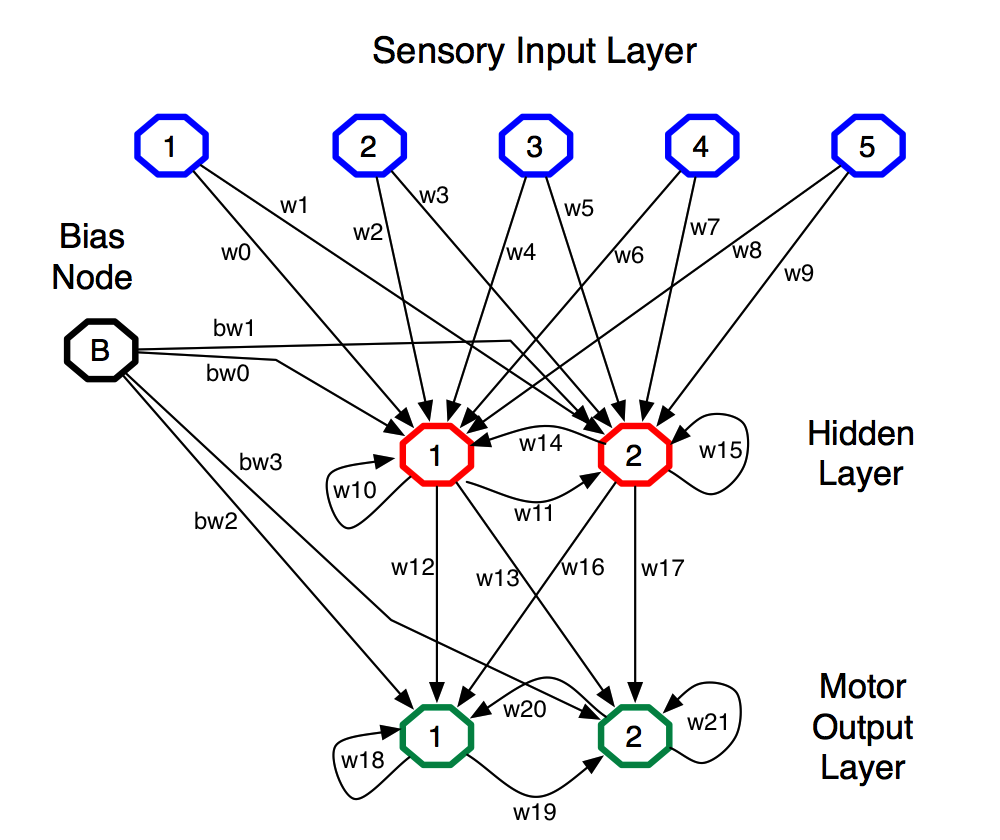
\includegraphics[width=1.0\textwidth]{img/CTRNN}
    \caption{The CTRNN network used in the Tracker agent}
\end{figure}

\begin{tabular}{c | c | c | c | c | c | c | c | c | c | c | c | c }

w0  & w1  & w2  & w3  & w4  & w5  & w6  & w7  & w8  & w9  & w10 & w11 & w12 \\
\hline
0.1 & 0.1 & 0.1 & 0.1 & 0.1 & 0.1 & 0.1 & 0.1 & 0.1 & 0.1 & 0.1 & 0.1 & 0.1 \\ \\

w13 & w14 & w15 & w16 & w17 & w18 & w19 & w20 & w21 & bw0 & bw1 & bw2 & bw3 \\
\hline
0.1 & 0.1 & 0.1 & 0.1 & 0.1 & 0.1 & 0.1 & 0.1 & 0.1 & 0.1 & 0.1 & 0.1 & 0.1 \\

\end{tabular}
